

%% this section contains XX problems
%%----------------------------------------


%% Jacobs 5 steps to a 5
%%------------------------------
\element{AP}{
\begin{question}{Jacobs-Q03}
    What is the vertical component of $\mathbf{F}_1$ in the
        diagram below?
    \begin{center}
        %% NOTE: Tikz diagram
        %\includegraphics[keepaspectratio]{Jacobs-Q03}
    \end{center}
    \begin{multicols}{3}
    \begin{choices}
        \wrongchoice{$\frac{1}{2}\mathbf{F}_1$}
        \wrongchoice{$\mathbf{F}_1$}
        \wrongchoice{$\mathbf{F}_1\cos\theta$}
      \correctchoice{$\mathbf{F}_1\sin\theta$}
        \wrongchoice{$\mathbf{F}_1\tan\theta$}
    \end{choices}
    \end{multicols}
\end{question}
}

\element{AP}{
\begin{question}{Jacobs-Q04}
    The box pictured below moves at constant speed to the left.
    \begin{center}
        %% NOTE: Tikz diagram
        %\includegraphics[keepaspectratio]{Jacobs-Q03}
    \end{center}
    Which of the following is correct?
    \begin{multicols}{3}
    \begin{choices}
        \wrongchoice{The situation is impossible.
            Because more forces act right, the block must move
            to the right.}
        \wrongchoice{$T_3 > T_1 + T_2$}
        \wrongchoice{$T_3 < T_1 + T_2$}
      \correctchoice{$T_3 = T_1 + T_2$}
        \wrongchoice{A relationship among the three tensions
            cannot be determined from the information given.}
    \end{choices}
    \end{multicols}
\end{question}
}

\element{AP}{
\begin{question}{Jacobs-Q04}
    The box pictured below moves at constant speed to the left.
    \begin{center}
        \includegraphics[keepaspectratio]{Jacobs-Q03}
    \end{center}
    Which of the following is correct?
    \begin{multicols}{3}
    \begin{choices}
        \wrongchoice{The situation is impossible.
            Because more forces act right, the block must move
            to the right.}
        \wrongchoice{$T_3 > T_1 + T_2$}
        \wrongchoice{$T_3 < T_1 + T_2$}
      \correctchoice{$T_3 = T_1 + T_2$}
        \wrongchoice{A relationship among the three tensions
            cannot be determined from the information given.}
    \end{choices}
    \end{multicols}
\end{question}
}

\element{AP}{
\begin{question}{Jacobs-Q05}
    A block of mass $m$ is sliding up a frictionless incline,
        as shown below.
    The block's initial velocity is \SI{3}{\meter\per\second}
        up the plane.
    \begin{center}
        \includegraphics[keepaspectratio]{Jacobs-Q03}
    \end{center}
    What is the component of the weight parallel to the plane?
    \begin{multicols}{3}
    \begin{choices}
        \wrongchoice{$mg$}
        \wrongchoice{$mg\cos\ang{40}$}
      \correctchoice{$mg\sin\ang{40}$}
        \wrongchoice{$g\sin\ang{40}$}
        \wrongchoice{$g\cos\ang{40}$}
    \end{choices}
    \end{multicols}
\end{question}
}

\element{AP}{
\begin{question}{Jacobs-Q05}
    A block of mass $m$ is sliding up a frictionless incline,
        as shown below.
    The block's initial velocity is \SI{3}{\meter\per\second}
        up the plane.
    \begin{center}
        \includegraphics[keepaspectratio]{Jacobs-Q03}
    \end{center}
    What is the acceleration of the mass?
    \begin{multicols}{3}
    \begin{choices}
        \wrongchoice{\SI{3}{\meter\per\second}, up the plane}
        \wrongchoice{$mg\sin\ang{40}$, up the plane}
        \wrongchoice{$mg\sin\ang{40}$, down the plane}
      \correctchoice{$g\sin\ang{40}$, up the plane}
        \wrongchoice{$g\sin\ang{40}$, down the plane}
    \end{choices}
    \end{multicols}
\end{question}
}

\element{AP}{
\begin{question}{Jacobs-APB-Q06}
    A block of mass $m$ sits on the ground.
    A student pulls up on the block with a tension $T$,
        but the block remains in contact with the ground.
    What is the normal force on the block?
    \begin{multicols}{3}
    \begin{choices}
        \wrongchoice{$T + mg$}
        \wrongchoice{$T - mg$}
        \wrongchoice{$mg$}
      \correctchoice{$mg - T$}
        \wrongchoice{$T$}
    \end{choices}
    \end{multicols}
\end{question}
}

\element{AP}{
\begin{question}{Jacobs-APB-Q09}
    A free-body diagram includes vectors representing the individual
        forces acting on an object.
    Which of these quantities should \emph{not} appear on a free-body diagram?
    \begin{choices}
        \wrongchoice{tension of a rope}
      \correctchoice{mass times acceleration}
        \wrongchoice{kinetic friction}
        \wrongchoice{static friction}
        \wrongchoice{weight}
    \end{choices}
\end{question}
}

\element{AP}{
\begin{question}{Jacobs-APB-Q10}
    An object rolls along level ground to the right at
        constant speed.
    Must there be any forces pushing this object to the right?
    \begin{choices}
        \wrongchoice{Yes: the \emph{only} forces that act must be to the right}
        \wrongchoice{Yes: but there could also be a friction force acting to the left}
        \wrongchoice{No: no forces can act to the right}
      \correctchoice{No: while there can be forces acting, no force \emph{must} act.}
        \wrongchoice{The answer depends on the speed of the object.}
    \end{choices}
\end{question}
}

\element{AP}{
\begin{question}{Jacobs-APB-Q11}
    A person stands on a scale in an elevator.
    He notices that the scale reading is lower than his usual weight.
    Which of the following could possibly describe the motion of the elevator?
    \begin{choices}
        \wrongchoice{It is moving down at constant speed.}
        \wrongchoice{It is moving down and slowing down.}
      \correctchoice{It is moving up and slowing down.}
        \wrongchoice{It is moving up and speeding up.}
        \wrongchoice{It is moving up at constant speed.}
    \end{choices}
\end{question}
}


%% 2004-APB
%%------------------------------
\element{AP}{
\begin{question}{2004-APB-Q02}
    A rope of negligible mass supports a block that weights \SI{30}{\newton},
        as shown below.
    \begin{center}
        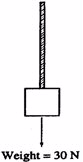
\includegraphics[keepaspectratio]{2004-APB-Q02}
    \end{center}
    The breaking strength of the rope is \SI{50}{\newton}.
    The largest acceleration that can be given to the block by pulling
        up on it with the rope without breaking the rope is most nearly
    \begin{multicols}{3}
    \begin{choices}
      \correctchoice{\SI{6}{\meter\per\second\squared}}
        \wrongchoice{\SI{6.7}{\meter\per\second\squared}}
        \wrongchoice{\SI{10}{\meter\per\second\squared}}
        \wrongchoice{\SI{15}{\meter\per\second\squared}}
        \wrongchoice{\SI{16.7}{\meter\per\second\squared}}
    \end{choices}
    \end{multicols}
\end{question}
}

\element{AP}{
\begin{question}{2004-APB-Q04}
    A ball is thrown straight up in the air.
    When the ball reaches its highest point,
        which of the following is true?
    \begin{choices}
      \correctchoice{None of the provided answer.}
        \wrongchoice{It is in equilibrium.}
        \wrongchoice{It has zero acceleration.}
        \wrongchoice{It has maximum momentum.}
        \wrongchoice{It has maximum kinetic energy.}
    \end{choices}
\end{question}
}

\element{AP}{
\begin{question}{2004-APB-Q05}
    The figure below shows an object of mass \SI{0.4}{\kilo\gram}
        that is suspended from a scale and submerged in a liquid.
    \begin{center}
        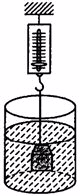
\includegraphics[keepaspectratio]{2004-APB-Q05}
    \end{center}
    If the reading on the scale is \SI{3.0}{\newton}, then
        the buoyant force that the fluid exerts on the object is most
        nearly
    \begin{multicols}{3}
    \begin{choices}
      \correctchoice{\SI{1.0}{\newton}}
        \wrongchoice{\SI{0.33}{\newton}}
        \wrongchoice{\SI{0.25}{\newton}}
        \wrongchoice{\SI{1.3}{\newton}}
        \wrongchoice{\SI{0.75}{\newton}}
    \end{choices}
    \end{multicols}
\end{question}
}

\element{AP}{
\begin{question}{2004-APB-Q11}
    The graph below represents position $x$ verses time $t$ for an object being
        acted on by a constant force.
    \begin{center}
        %% replace with pgfplots
        %\includegraphics[keepaspectratio]{2004-APB-Q11}
    \end{center}
    The average speed during the interval between \SI{1}{\second} and \SI{2}{\second}
        is most nearly
    \begin{multicols}{3}
    \begin{choices}
        \wrongchoice{\SI{2}{\newton}}
        \wrongchoice{\SI{4}{\newton}}
        \wrongchoice{\SI{5}{\newton}}
      \correctchoice{\SI{6}{\newton}}
        \wrongchoice{\SI{8}{\newton}}
    \end{choices}
    \end{multicols}
\end{question}
}

\element{AP}{
\begin{question}{2004-APB-Q29}
    A student obtains data on the magnitude of force applied to an object as
        a function of time and displays the data on the graph below.
    \begin{center}
        %% Replace with pgfplots
        %\includegraphics[keepaspectratio]{2004-APB-Q29}
    \end{center}
    The slope of the ``best fit'' straight line is most near
    \begin{multicols}{3}
    \begin{choices}
      \correctchoice{\SI{5.0}{\newton\per\second}}
        \wrongchoice{\SI{6.0}{\newton\per\second}}
        \wrongchoice{\SI{7.0}{\newton\per\second}}
        \wrongchoice{\SI{8.0}{\newton\per\second}}
        \wrongchoice{\SI{10}{\newton\per\second}}
    \end{choices}
    \end{multicols}
\end{question}
}

\element{AP}{
\begin{question}{2004-APB-Q30}
    A student obtains data on the magnitude of force applied to an object as
        a function of time and displays the data on the graph below.
    \begin{center}
        %% Replace with pgfplots
        \includegraphics[keepaspectratio]{2004-APB-Q29}
    \end{center}
    The increase in the momentum of the object between $t=\SI{0}{\second}$ and
        $t=\SI{4}{\second}$ is most nearly
    \begin{multicols}{3}
    \begin{choices}
        \wrongchoice{\SI{40}{\newton\second}}
        \wrongchoice{\SI{50}{\newton\second}}
      \correctchoice{\SI{60}{\newton\second}}
        \wrongchoice{\SI{80}{\newton\second}}
        \wrongchoice{\SI{100}{\newton\second}}
    \end{choices}
    \end{multicols}
\end{question}
}

\element{AP}{
\begin{question}{2004-APB-Q31}
    How does an air mattress protect a stunt person landing on the ground
        after a stunt?
    \begin{choices}
        \wrongchoice{It reduced the kinetic energy loss of the stunt person.}
        \wrongchoice{It reduced the momentum change of the stunt person.}
        \wrongchoice{It increases the momentum change of the stunt person.}
        \wrongchoice{It shortens the stopping time of the stunt person and
                        increase the force applied during the landing.}
      \correctchoice{It lengthens the stopping time of the stunt person and
                        reduces the force applied during the landing.}
    \end{choices}
\end{question}
}

%% NOTE: alt1 just direction
%% NOTE: alt2 both magnitude and direction 
%% Answer is 0.5 m/s^2 to the left
\element{AP}{
\begin{question}{2004-APB-Q41}
    The cart of mass \SI{10}{\kilo\gram} shown below moves without
        frictional loss on a level table.
    \begin{center}
        \includegraphics[keepaspectratio]{2004-APB-Q41}
    \end{center}
    A \SI{10}{\newton} force pulls on the cart horizontally to the
        right.
    At the same time, a \SI{30}{\newton} force at an angle of \ang{60}
        above the left.
    What is the magnitude of the horizontal acceleration of the cart?
    \begin{multicols}{3}
    \begin{choices}
      \correctchoice{\SI{0.5}{\meter\per\second\squared}}
        \wrongchoice{\SI{1.6}{\meter\per\second\squared}}
        \wrongchoice{\SI{2.0}{\meter\per\second\squared}}
        \wrongchoice{\SI{2.5}{\meter\per\second\squared}}
        \wrongchoice{\SI{2.6}{\meter\per\second\squared}}
    \end{choices}
    \end{multicols}
\end{question}
}

